\documentclass[../DS08.tex]{subfiles}%
\graphicspath{{./figures/}}%

% \subimport{/home/nora/Documents/Enseignement/Prepa/bpep/exercices/DS/titrage_CO2/}{sujet.tex}%

\begin{document}%
\section[43]"E"{Dioxyde de carbone en solution aqueuse}

\subsection{Les pluies acides}%
\enonce{
	Le dioxyde de carbone gazeux \ce{CO2(g)} a un caractère acide. Il réagit avec l'eau pour former \og{}l'acide carbonique\fg{} que nous noterons \ce{CO2(aq)}. On considère de l'eau de pluie en équilibre avec le \ce{CO2(g)} de l'atmosphère à \SI{298}{K}, la pression totale étant de \SI{1}{bar} et la pression partielle en \ce{CO2(g)} étant $P(\ce{CO2(g)})=\SI{35e-5}{bar}$.

	La concentration de \ce{CO2(aq)} dans l'eau de pluie vaut \SI{1.19e-5}{mol.L^{-1}}.

	Données :
	\begin{itemize}%
		\item Couple \ce{CO2(aq) / HCO^-_3(aq)} : $\p K_{a_1}=6,3$
		\item Couple \ce{HCO^-_3(aq) / CO^{2-}_3(aq)} : $\p K_{a_2}=10,3$
	\end{itemize}
}%

\QR[2]{\label{Q:diagramme}%
	Sur une même échelle en pH, représenter le diagramme de prédominance du dioxyde de carbone et de ses composés dérivés.
}{%
	\begin{center}%
		% \begin{tikzpicture}[scale=0.75]
		% 	\draw[->,>=latex] (0,0) -- (14,0) ;
		% 	\draw (6.3,0) -- (6.3,2) ;
		% 	\draw (10.3,0) -- (10.3,2) ;
		% 	\draw (14,0) node[right]{pH} ;
		% 	\draw (6.3,0) node[below] {$\p K_{a_1}=6,3$} ;
		% 	\draw (10.3,0) node[below] {$\p K_{a_2}=10,3$} ;
		% 	\draw (3.15,1) node{\ce{CO2(aq)}} ;
		% 	\draw (8.3,1) node{\ce{HCO^-_3(aq)}} ;
		% 	\draw (12.15,1) node{\ce{CO^{2-}_3(aq)}} ;
		% \end{tikzpicture}%
		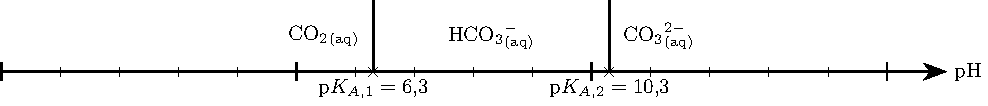
\includegraphics[scale=1]{predom_co2}
	\end{center}%
}%

\QR[10]{%
Calculer le pH de l'eau de pluie, en considérant que le dioxyde de carbone est
le seul responsable de la valeur que prend le pH de l'eau de pluie. Pour ce
calcul, on pourra émettre l'hypothèse que l'on peut n'envisager que la
première acidité. On vérifiera \textit{a posteriori} cette hypothèse.
}{%
\leavevmode\vspace*{-15pt}\relax
\begin{center}
	\def\rhgt{0.35}
	\centering
	\begin{tabularx}{.8\linewidth}{|l|c||YdYdYdY|}
		\hline
		\multicolumn{2}{|c||}{
			$\xmathstrut{\rhgt}$
		\textbf{Équation}}           &
		$\ce{{CO_2}_{\aqu}}$         & $+$              &
		$2\ce{{H_2O}_{\liq}}$        & $=$              &
		$\ce{{HCO_3}^-_{\aqu}}$      & $+$              &
		$\ce{{H_3O}^+_{\aqu}}$\tikzmark{EP0}              \\
		\hline
		$\xmathstrut{\rhgt}$
		Initial                      & $x = 0$          &
		$c_0$                        & \vline           &
		excès                        & \vline           &
		$0$                          & \vline           &
		$0$                                               \\
		\hline
		$\xmathstrut{\rhgt}$
		Final                        & $x_f = x_{\equ}$ &
		$c_0 - x_{\equ} \approx c_0$ & \vline           &
		excès                        & \vline           &
		$x_{\equ}$                   & \vline           &
		$x_{\equ}$ \tikzmark{RP0}                         \\
		\hline
	\end{tabularx}
\end{center}
\tikz[remember picture, overlay]
\node[right=20pt of pic cs:EP0] {\pt{1}+\pt{1}};
\tikz[remember picture, overlay]
\node[above right=3pt and 30pt of pic cs:RP0] {\pt{1}};

Comme $K_{a_1}\ll 1$, on peut faire l'hypothèse d'une réaction faiblement
avancée, soit $x\ind{eq}\ll c_0 \pt{1} = \SI{1.19e-5}{mol.L^{-1}}$.
\begin{gather*}
	\beforetext{Loi d'action de masse}
	K_{a_1}\stm{\approx}
	\cfrac{x\ind{eq}^2}{c_0c^\circ}
	\qsoit
	\boxed{x\ind{eq} \stm{\approx} \sqrt{c^\circ c_0K_{a_1}}}
	\Lra
	\xul{x\ind{eq} \stm{=} \SI{2.44e-6}{mol.L^{-1}}}
	\\\beforetext{D'où}
	\boxed{\pH = -\log(\frac{x\ind{eq}}{c^\circ})}
	\Ra \xul{\pH \stm{=} \num{5,6}}
\end{gather*}

On vérifie que la valeur de pH obtenue appartient bien au domaine de
prédominance de \ce{CO2}, \pt{1} d'où la validité d'une réaction faiblement
avancée.

De plus, ce pH est très éloigné du domaine de prédominance de \ce{CO_3^{2-}},
donc cette espèce est minoritaire \pt{1}. Cette constatation est cohérente avec
l'hypothèse de ne considérer que la première acidité du dioxyde de carbone.
}%

\subsection{Le dioxyde de carbone au laboratoire}%

\QR[3]{%
	Donner la position de l'hydrogène, du carbone et de l'oxygène dans le tableau
	périodique. Préciser leur nombre d'électrons de valence. On donne les numéros
	atomiques~:
	\[
		\ce{H}:Z=1\quad ;\quad \ce{C}:Z=6\quad ;\quad \ce{O} : Z=8
	\]
}{%
	\leavevmode\vspace*{-20pt}\relax
	\begin{itemize}[leftmargin=20pt]%
		\item[l][15]{\pt{1}}%
		\ce{H}~: première ligne première colonne, 1 électron de valence.
		\item[l][15]{\pt{1}}%
		\ce{C}~: deuxième ligne et deuxième colonne du bloc $p$, 4 électrons
		de valence.
		\item[l][15]{\pt{1}}%
		\ce{O}~: deuxième ligne et seizième colonne, 6 électrons de valence.
	\end{itemize}%
}%

\QR[3]{%
	Donner une représentation de Lewis de la molécule de dioxyde de carbone
	\ce{CO2}, et des ions hydrogénocarbonate \ce{HCO^-_3} et carbonate
	\ce{CO^{2-}_3}.
}{%
	\leavevmode\vspace*{-15pt}\relax
	\hspace*{\fill}
	\begin{center}%
		\begin{tabular}{*{3}{p{0.3\linewidth}}}%
			\chemfig{
			\charge{135=\|,-135=\|}{O}
				=[0,0.6]
			\charge{90:10pt={\pt{1}}}{C}
					=[0,0.6]
				\charge{45=\|,-45=\|}{O}
			} &
			\chemfig{
			H-[0,0.6]\charge{90=\|,-90=\|}{O}
			-[0,0.6]
			\charge{-90:10pt={\pt{1}}}{C}
			(-[90,0.6]\chemabove{\charge{0=\|,90=\|,180=\|}{O}}{\hspace*{-0.7cm}\ominus})
			=[0,0.6]\charge{45=\|,-45=\|}{O}%
			}%
			  &
			\chemfig{
			\chemabove{\charge{180=\|,90=\|,-90=\|}{O}}{\hspace*{-0.7cm}\ominus}-[0,0.6]
			\charge{-90:10pt={\pt{1}}}{C}
			(-[90,0.6]\chemabove{\charge{0=\|,90=\|,180=\|}{O}}{\hspace*{-0.7cm}\ominus})
			=[0,0.6]\charge{45=\|,-45=\|}{O}%
			}   \\
		\end{tabular}%
	\end{center}%
}%

\QR[7]{%
En vous aidant du diagramme établi à la question \ref{Q:diagramme}, calculer
les concentrations molaires en \ce{CO2(aq)}, \ce{HCO^-_3(aq)} et
\ce{CO^{2-}_3(aq)} contenues dans des solutions tamponnées de \SI{1.0}{L} à un
pH donné (cf.\ tableau ci-dessous) quand on y a introduit \SI{0.10}{mol} de
\ce{CO2(aq)}. Vous recopierez le tableau ci-dessous et le complèterez.
\begin{center}%
	\begin{tabular}{*{6}{|c}|}%
		\hline
		pH                                          & 2             & 6,3           & 8             & 10,3          & 14            \\
		\hline
		$[\ce{CO2(aq)}]\ind{eq}$ en \si{mol.L^-1}   & \hspace*{1cm} & \hspace*{1cm} & \hspace*{1cm} & \hspace*{1cm} & \hspace*{1cm} \\
		\hline
		$[\ce{HCO^-_3}]\ind{eq}$ en \si{mol.L^-1}   &               &               &               &               &               \\
		\hline
		$[\ce{CO^{2-}_3}]\ind{eq}$ en \si{mol.L^-1} &               &               &               &               &               \\
		\hline
	\end{tabular}%
\end{center}%
}{%
On exploite la conservation de la matière
\begin{gather*}
	[\ce{CO2(aq)}]\ind{eq} + [\ce{HCO^-_3}]\ind{eq} + [\ce{HCO^{2-}_3}]\ind{eq}
	\stm{=} C_0 % = \SI{0.1}{mol.L^{-1}}
	\tag{0}
	\label{eq:0}
\end{gather*}
ainsi que les relations entre le pH et les constantes d'acidité
\begin{align*}
	\pH & \stm(un){=}\p K_{a_1} +\log\pa{\cfrac{[\ce{HCO^-_3}]\ind{eq}}{[\ce{CO2(aq)}]\ind{eq}}}
	\tag{1}
	\label{eq:1}
	\\
	\pH & =\p K_{a_2} +\log\pa{\cfrac{[\ce{CO^{2-}_3}]\ind{eq}}{[\ce{HCO^-_3}]\ind{eq}}}
	\tag{2}
	\label{eq:2}
\end{align*}

Le diagramme de prédominance va nous aider à simplifier ce système de 3 équations
à 3 inconnues.

\begin{itemize}%
	\item[l][15]{\pt{1}}%
	Pour $\pH=2$, \ce{CO2} prédomine. On fait alors
	l'hypothèse que $[\ce{CO2(aq)}]\ind{eq}\approx C_0$ (d'après
	l'équation~\eqref{eq:0}). L'équation~\eqref{eq:1} donne
	\begin{gather*}
		[\ce{HCO^-_3}]\ind{eq} =
		[\ce{CO2(aq)}]\ind{eq}\times 10^{\pH-\p K_{a_1}}
		\qsoit
		\xul{[\ce{HCO^-_3}]\ind{eq}=\SI{5,0e-6}{mol.L^{-1}}}%
	\end{gather*}
	L'équation~\eqref{eq:2} donne
	\[
		[\ce{CO^{2-}_3}]\ind{eq} =
		[\ce{HCO^-_3}]\ind{eq}\times 10^{\pH-\p K_{a_2}}
		\qsoit
		\xul{[\ce{CO^{2-}_3}]\ind{eq}=\SI{2.5e-14}{mol.L^{-1}}}
	\]
	\item[l][15]{\pt{1}}%
	Pour $\pH=6,3=\p K_{a_1} $, $[\ce{CO2(aq)}]\ind{eq}=[\ce{HCO^-_3}]\ind{eq} =
		C_0/2 = \SI{5.0e-2}{mol.L^{-1}}$ et on en déduit la concentration en ion
	carbonate à l'aide de l'équation~\eqref{eq:2} :
	\[
		[\ce{CO^{2-}_3}]\ind{eq}=
		[\ce{HCO^-_3}]\ind{eq}\times 10^{\pH-\p K_{a_2}}
		\qsoit
		\xul{[\ce{HCO^-_3}]\ind{eq}=\SI{5.0e-6}{mol.L^{-1}}}
	\]

	\item[l][15]{\pt{1}}%
	Pour $\pH=8$, \ce{HCO^-_3} prédomine. On fait alors l'hypothèse que
	$[\ce{HCO^-_3}]\ind{eq}\approx C_0$ (d'après l'équation~\eqref{eq:0}).
	L'équation~\eqref{eq:1} donne
	\[
		[\ce{CO2(aq)}]\ind{eq} =
		[\ce{HCO^-_3}]\ind{eq}\times 10^{\p K_{a_1}-\pH}
		\qsoit
		\xul{[\ce{CO2(aq)}]\ind{eq}=\SI{2.0e-3}{mol.L^{-1}}}
	\]
	L'équation~\eqref{eq:2} donne
	\[
		[\ce{CO^{2-}_3}]\ind{eq} =
		[\ce{HCO^-_3}]\ind{eq}\times 10^{\pH-\p K_{a_2}}
		\qsoit
		\xul{[\ce{CO^{2-}_3}]\ind{eq}=\SI{5.0e-4}{mol.L^{-1}}}
	\]
	\item[l][15]{\pt{1}}%
	Pour $\pH=10,3=\p K_{a_2}$, $[\ce{CO^{2-}_3}]\ind{eq} =
		[\ce{HCO^-_3}]\ind{eq} = C_0/2 = \SI{5.0e-2}{mol.L^{-1}}$ et on en déduit la
	concentration en ion carbonate à l'aide de l'équation~\eqref{eq:1} :
	\[
		[\ce{CO2(aq)}]\ind{eq} =
		[\ce{HCO^-_3}]\ind{eq}\times 10^{\p K_{a_1}-\pH}
		\qsoit
		\xul{[\ce{CO2(aq)}]\ind{eq}=\SI{5.0e-6}{mol.L^{-1}}}
	\]
	\item[l][15]{\pt{1}}%
	Pour $\pH=14$, \ce{CO^{2-}_3} prédomine. On fait alors l'hypothèse que
	$[\ce{CO^{2-}_3}]\ind{eq}\approx C_0$ (d'après l'équation~\eqref{eq:0}).
	L'équation~\eqref{eq:2} donne
	\[
		[\ce{HCO^-_3}]\ind{eq} =
		[\ce{CO^{2-}_3}]\ind{eq}\times 10^{\p K_{a_2}-\pH}
		\qsoit
		\xul{[\ce{HCO^-_3}]\ind{eq}=\SI{2.0e-5}{mol.L^{-1}}}%
	\]
	L'équation~\eqref{eq:1} donne
	\[
		[\ce{CO2(aq)}]\ind{eq} =
		[\ce{HCO^-_3}]\ind{eq}\times 10^{\p K_{a_1}-\pH}
		\qsoit
		\xul{[\ce{CO2(aq)}]\ind{eq}=\SI{4.0e-13}{mol.L^{-1}}}
	\]
\end{itemize}%
{\begin{center}%
	\begin{tabular}{*{6}{|c}|}%
		\hline
		pH                                          & 2             & 6,3          & 8            & 10,3         & 14            \\
		\hline
		$[\ce{CO2(aq)}]\ind{eq}$ en \si{mol.L^-1}   & \num{1.0e-1}  & \num{5.0e-2} & \num{2.0e-3} & \num{5.0e-6} & \num{4.0e-13} \\
		\hline
		$[\ce{HCO^-_3}]\ind{eq}$ en \si{mol.L^-1}   & \num{5.0e-6}  & \num{5.0e-2} & \num{1.0e-1} & \num{5.0e-2} & \num{2.0e-5}  \\
		\hline
		$[\ce{CO^{2-}_3}]\ind{eq}$ en \si{mol.L^-1} & \num{2.5e-14} & \num{5.0e-6} & \num{5.0e-4} & \num{5.0e-2} & \num{1.0e-1}  \\
		\hline
	\end{tabular}%
\end{center}}%
}%

\enonce{%
	Une solution de soude de concentration $C_B$ a été abandonnée dans un
	laboratoire pendant plusieurs jours, dans un flacon débouché de volume
	$V\ind{tot}=\SI{1}{L}$. Lorsqu'on récupère le flacon, on décide de doser un
	volume $V_0=\SI{20}{mL}$ de la solution contenue dans le flacon par de l'acide
	chlorhydrique de concentration $C_A=\SI{1.00e-1}{mol.L^{-1}}$.
	\bigbreak
	Le suivi pH-métrique donne la courbe qui suit. Il apparait sur cette courbe
	deux points d'inflexion correspondant aux volumes $V_1=\SI{15.8}{mL}$ et
	$V_2=\SI{20.1}{mL}$ d'acide chlorhydrique versé.
	\bigbreak
	On donne aussi le diagramme de distribution en fonction du pH pour les espèces
	\ce{CO2(aq)}, \ce{HCO^-_3} et \ce{CO^{2-}_3}.

	\noindent
	\begin{minipage}[t]{.48\linewidth}
		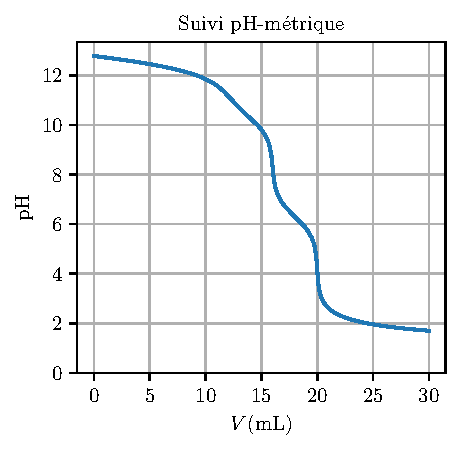
\includegraphics[width=\linewidth]{graphe_pH}%
	\end{minipage}
	\hfill
	\begin{minipage}[t]{.48\linewidth}
		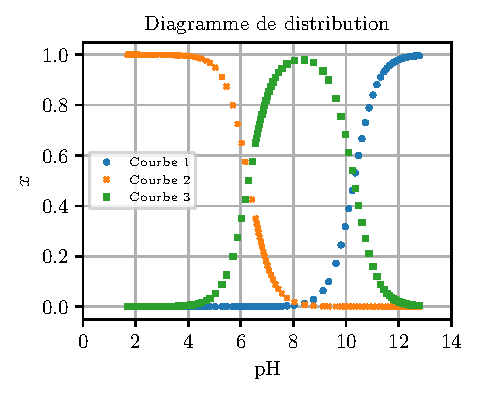
\includegraphics[width=\linewidth]{graphe_distribution}%
	\end{minipage}
}%

\QR[2]{%
	Quelles sont les espèces présentes dans la solution avant le titrage ?
}{%
	La solution de soude est composée des ions \ce{Na+} et \ce{HO-} \pt{1}.
	Le dioxyde de carbone de l'air s'est dissous dans la solution. Comme le pH
	initial vaut 13, le dioxyde de carbone dissous se trouve sous la forme
	\ce{CO^{2-}_3}. Il y a bien sûr de l'eau \ce{H2O}. \pt{1}
}%

\QR[10]{%
	Quelles sont les réactions susceptibles de se produire au cours du titrage~?
	On précisera la valeur des constantes d'équilibre, et on analysera les valeurs
	de ces constantes au regard de la courbe de titrage et du diagramme de
	distribution donnés. Indiquer notamment lesquelles sont successives ou non.
}{%
	\noindent
	\begin{minipage}[t]{.78\linewidth}
		On trace une échelle en $\pk$. Initialement, il peut y avoir deux réactions~:
		\begin{align*}
			\beforetext{$K_1 = 10^{14}$}
			\ce{HO^-_{\aqu} + H3O^+_{\aqu}           & \stm{=} 2H2O_{\liq}}
			\tag*{R1}
			\label{eq:R1}
			\\
			\beforetext{$K_2 \stm{=} 10^{10,3}$}
			\ce{{CO_3}^{2-}_{\aqu} + {H_3O}^+_{\aqu} & \stm{=} {HCO_3}^-_{\aqu} + H2O_{\liq}}
			\tag*{R2}
			\label{eq:R2}
		\end{align*}
		Ces deux réactions sont totales \pt{1}, mais comme $K_1/K_2\approx 10^4$, on
		n'est pas sûrx que les titrages soient successifs. Pour cela, on lit le pH à
		la première équivalence~: $\pH (V_1)\approx 8$ \pt{1}. D'après le diagramme
		de distribution, $[\ce{CO^{2-}_3}]\ll [\ce{HCO^-_3}]$ et $[\ce{CO2(aq)}]\ll
			[\ce{HCO^-_3}]$. Ainsi la réaction~\eqref{eq:R2} est finie au volume d'acide
		$V_1$ versé. Donc les réactions~\eqref{eq:R1} et \eqref{eq:R2} se font
		simultanément \pt{1}.
	\end{minipage}
	\hfill
	\begin{minipage}[t]{.20\linewidth}
		\vspace{0pt}
		\begin{center}
			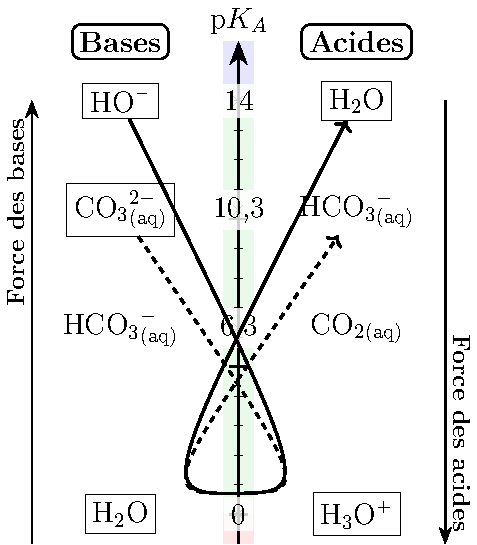
\includegraphics[width=\linewidth]{echpka_co2-a}
			\captionof*{figure}{\footnotesize Début du titrage \protect\pt{1}}
		\end{center}
	\end{minipage}
	\noindent
	\begin{minipage}[c]{.20\linewidth}
		\begin{center}
			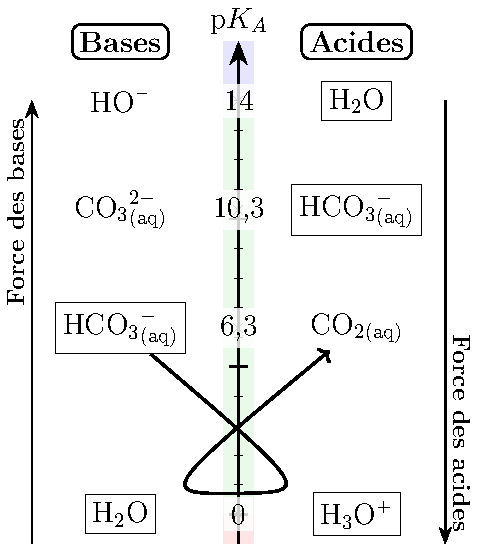
\includegraphics[width=\linewidth]{echpka_co2-b}
			\captionof*{figure}{\footnotesize Fin du titrage \protect\pt{2}}
		\end{center}
	\end{minipage}
	\hfill
	\begin{minipage}[c]{.78\linewidth}
		La deuxième réaction de titrage forme \ce{HCO^-_3} qui est une base faible.
		Elle peut donc réagir avec \ce{H3O+} selon la réaction
		\[
			\beforetext{$K_3 = 10^{6,3}$}
			\ce{{HCO_3}^{-}_{\aqu} + {H_3O}^+_{\aqu} \stm{=} CO2_{\aqu} + 2H2O_{\liq}}
			\tag*{R3}
			\label{eq:R3}
		\]
		Cette réaction est quantitative. Elle se produit après les deux autres,
		\pt{1} pour $V\in[V_1,V_2]$.
	\end{minipage}
}%

\QR[6]{%
En déduire la concentration $C_B$ de la solution de soude et la quantité de
matière de dioxyde de carbone dissous dans le flacon de volume
$V\ind{tot}=\SI{1.00}{L}$.
}{%
D'après la réaction de titrage~\eqref{eq:R3}, en notant $[\ce{CO2}]$ la
concentration de dioxyde de carbone dissous dans le flacon :
\[
	C_A(V_2-V_1) \stm{=}\ [\ce{CO_2}] V_0
	\qsoit
	[\ce{CO_2}] \stm{=} \SI{2.15e-2}{mol.L^{-1}}
\]
On en déduit la quantité dans le volume total
\[
	\boxed{n(\ce{CO2})\ind{tot} \stm{=}\ [\ce{CO_2}]\times V\ind{tot}}
	\qsoit
	\xul{n(\ce{CO2})\ind{tot} \stm{=} \SI{21.5}{mmol}}
\]
Pour déterminer la concentration en \ce{HO-}, on utilise la première
équivalence. Les réactions de titrage~\eqref{eq:R1} et \eqref{eq:R2} se faisant
simultanément, on dose la quantité de soude et celle de dioxyde de carbone
dissous. La relation à l'équivalence s'écrit
\[
	C_AV_1 = (C_B+[\ce{CO2}])V_0
	\qsoit
	\boxed{C_B \stm{=} \cfrac{C_AV_1}{V_0}-[\ce{CO2}]}
	\Ra
	\xul{C_B \stm{=} \SI{5.75e-2}{mol.L^{-1}}}
\]
}%

\end{document}%
